\documentclass[border=4pt]{standalone}
\usepackage[compat=1.1.0]{tikz-feynman}
\tikzfeynmanset{every vertex={dot}, every blob={draw}}
\begin{document}
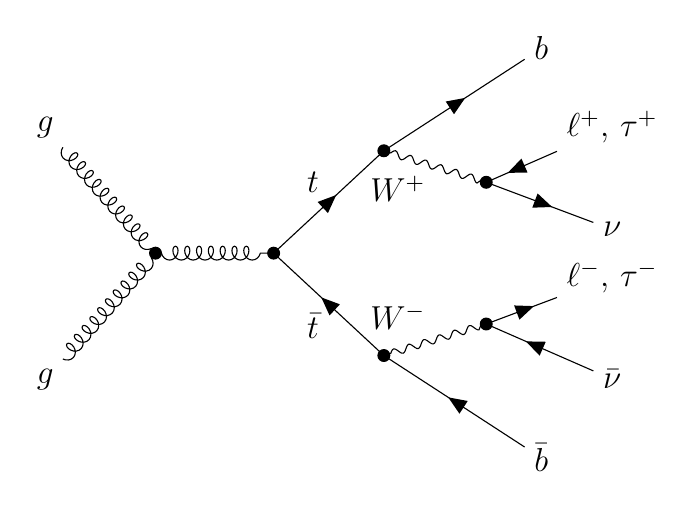
\begin{tikzpicture}[font=\large]
\begin{feynman}
\vertex (g1) at (0, 1.6) {\(g\)};
\vertex (g2) at (0,-1.6) {\(g\)};
\vertex [dot] (a) at (1.4, 0) {};
\vertex [dot] (b) at (2.9, 0) {};
\vertex [dot] (t) at (4.3, 1.3) {};
\vertex [dot] (tb) at (4.3,-1.3) {};
\vertex (bq) at (6.3, 2.6) {\(b\)};
\vertex [dot] (w1) at (5.6, 0.9) {};
\vertex (l1) at (7.2, 1.6) {\(\ell^{+},\,\tau^{+}\)};
\vertex (n1) at (7.2, 0.3) {\(\nu\)};
\vertex (bbq) at (6.3,-2.6) {\(\bar{b}\)};
\vertex [dot] (w2) at (5.6,-0.9) {};
\vertex (l2) at (7.2,-0.3) {\(\ell^{-},\,\tau^{-}\)};
\vertex (n2) at (7.2,-1.6) {\(\bar{\nu}\)};
\diagram*{
 (g1) -- [gluon] (a),
 (g2) -- [gluon] (a),
 (a) -- [gluon] (b),
 (b) -- [fermion, edge label=\(t\)] (t),
 (tb) -- [fermion, edge label=\(\bar{t}\)] (b),
 (t) -- [fermion] (bq),
 (bbq) -- [fermion] (tb),
 (t) -- [boson, edge label'=\(W^{+}\)] (w1),
 (tb) -- [boson, edge label=\(W^{-}\)] (w2),
 (w1) -- [anti fermion] (l1),
 (w1) -- [fermion] (n1),
 (w2) -- [fermion] (l2),
 (w2) -- [anti fermion] (n2),
};
\end{feynman}
\end{tikzpicture}
\end{document}
